% !TEX root = ../main.tex

\clearpage
% Source PDF page 12.
\section{第六章\quad 奶蛙的衍生语与衍生动作}

奶蛙产生了许多奇妙的衍生语（绝大多数来源于王者荣耀中不知火舞语音的变速变调）和衍生动作。我们将会一一说明并提及有关的著名奶蛙二创作品。

\subsection{一、衍生语——安迪}

主要运用场景为爬行奶龙说话效果、奶蛋说话效果、奶蛙出场说话效果等，奶蛙高频说话效果之一。等效空耳有“俺滴”“安定”“俺无敌”“暗地”等。

\subsection{二、衍生语——嘎嘎滴辣虾}

运用场景广泛，奶蛙高频说话效果之一。等效空耳为“刚刚点了谁”“刚刚跌落水”“刚刚掉了什”等。

\subsection{三、衍生语——卡脚先}

主要运用场景为奶蛙小剧场的转折或收尾。等效空耳为“刚救下”“赶紧写”“干啥先”“啃脚先”等。

\subsection{四、衍生语——无了}

主要运用场景为奶蛙吃瘪、惊讶音效。等效空耳为“哦了”“好了”等。~(见\figref{fig:06-1})

% !TEX root = ../../main.tex
\begin{figure}[H]
  \centering
  
\includegraphics[width=128bp,height=0.76\textheight,keepaspectratio]{figures/chapter06/figure06_1.pdf}
  \renewcommand{\thefigure}{6.1}
  \caption{常伴随无了的奶蛙抱头动作}
  \label{fig:06-1}
\end{figure}


\subsection{五、衍生语——甘巴爹}

主要运用场景为奶蛙肯定、疑问音效。等效空耳为“干扒地”“刚拔的”等。

\subsection[六、衍生语——有用不]{六、衍生语——有用不~(见\figref{fig:06-2})}

主要用途为丰富奶蛙的语言，一般作为安迪的下位替代。等效空耳为“忧郁菇”“犹豫不”等。

% !TEX root = ../../main.tex
\begin{figure}[H]
  \centering
  
\includegraphics[width=55bp]{figures/chapter06/figure06_2.png}
  \renewcommand{\thefigure}{6.2}
  \caption{有用不？}
  \label{fig:06-2}
\end{figure}


\subsection[七、衍生动作——思考与抱胸]{七、衍生动作——思考与抱胸~(见\figref{fig:06-3})}

% !TEX root = ../../main.tex
\begin{figure}[H]
  \centering
  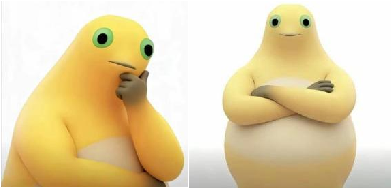
\includegraphics[width=84.8bp,height=0.76\textheight,keepaspectratio]{figures/chapter06/figure06_3.pdf}
  \renewcommand{\thefigure}{6.3}
  \caption{蹲起大笑的奶蛙}
  \label{fig:06-3}
\end{figure}


\clearpage
\subsection{八、衍生动作——蹲起大笑}

% !TEX root = ../../main.tex
\begin{figure}[H]
  \centering
  
\includegraphics[height=70bp]{figures/chapter06/figure06_4.pdf}\qquad
  
\includegraphics[height=70bp]{figures/chapter06/seasideLaughter.png}
  \renewcommand{\thefigure}{6.4}
  \caption{单人蹲起大笑（左）与海边双人大笑（右）}
  \label{fig:06-4}
\end{figure}


% Source PDF page 13.
熟悉蹲起大笑的人肯定知道，蹲起大笑还有双人组合技甚至多人组合技——因为画面过于神圣和有伤风化，我们按下不表（你只是怕了）。~(见\figref{fig:06-4})

\subsection{九、衍生动作——爬行}

% !TEX root = ../../main.tex
\begin{figure}[H]
  \centering
  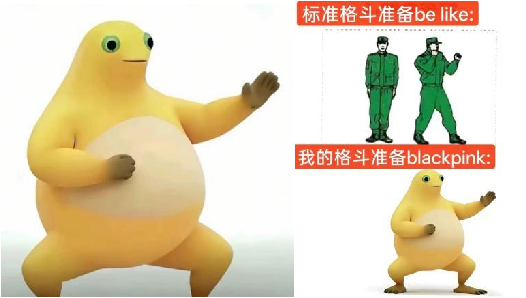
\includegraphics[width=111.32bp,height=0.76\textheight,keepaspectratio]{figures/chapter06/figure06_5.pdf}
  \renewcommand{\thefigure}{6.5}
  \caption{正在爬行前进的奶蛙}
  \label{fig:06-5}
\end{figure}


爬行奶蛙在爬到一半时会看向屏幕，说出一声“安迪”，然后继续爬行。~(见\figref{fig:06-5})

\subsection{十、衍生动作——摆架势}

% !TEX root = ../../main.tex
\begin{figure}[H]
  \centering
  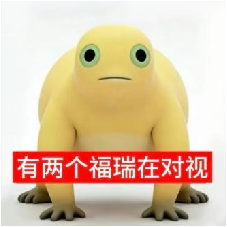
\includegraphics[width=92.55bp,height=0.76\textheight,keepaspectratio]{figures/chapter06/figure06_6.pdf}
  \renewcommand{\thefigure}{6.6}
  \caption{和读者对视的奶蛙}
  \label{fig:06-6}
\end{figure}


奶蛙的招牌动作之一。模仿奶蛙的青年们最常摆这个动作。~(见\figref{fig:06-6})

\clearpage
\subsection{十一、衍生动作——对视}

% !TEX root = ../../main.tex
\begin{figure}[H]
  \centering
  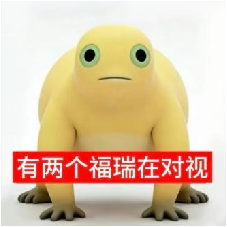
\includegraphics[width=93.77bp,height=0.76\textheight,keepaspectratio]{figures/chapter06/figure06_7.pdf}
  \renewcommand{\thefigure}{6.7}
  \caption{正在打坐的奶蛙}
  \label{fig:06-7}
\end{figure}


谁说奶蛙不是福瑞？奶蛙作为动物，很好的融入了“有两个福瑞在对视”的梗图，并且难绷程度青出于蓝。~(见\figref{fig:06-7})

\subsection[十二、衍生动作——打坐]{十二、衍生动作——打坐~(见\figref{fig:06-8})}

% !TEX root = ../../main.tex
\begin{figure}[H]
  \centering
  
\includegraphics[width=85.31bp,height=0.76\textheight,keepaspectratio]{figures/chapter06/figure06_8.pdf}
  \renewcommand{\thefigure}{6.8}
  \caption{正在魅惑读者的奶蛙}
  \label{fig:06-8}
\end{figure}


% Source PDF page 14.
\subsection[十三、衍生动作——魅惑]{十三、衍生动作——魅惑~(见\figref{fig:06-9})}

% !TEX root = ../../main.tex
\begin{figure}[H]
  \centering
  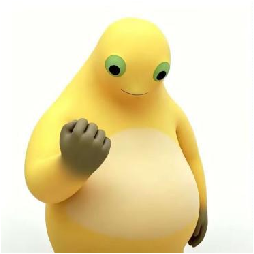
\includegraphics[width=103.67bp,height=0.76\textheight,keepaspectratio]{figures/chapter06/figure06_9.pdf}
  \renewcommand{\thefigure}{6.9}
  \caption{低头握拳的奶蛙}
  \label{fig:06-9}
\end{figure}


\clearpage
\subsection[十四、衍生动作——低头握拳]{十四、衍生动作——低头握拳~(见\figref{fig:06-10})}

% !TEX root = ../../main.tex
\begin{figure}[H]
  \centering
  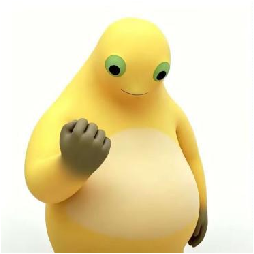
\includegraphics[width=103.67bp,height=0.76\textheight,keepaspectratio]{figures/chapter06/figure06_10.pdf}
  \renewcommand{\thefigure}{6.10}
  \caption{低头握拳的奶蛙}
  \label{fig:06-10}
\end{figure}


\subsection[十五、衍生动作——啃脚]{十五、衍生动作——啃脚~(见\figref{fig:06-11})}

% !TEX root = ../../main.tex
\begin{figure}[H]
  \centering
  
\includegraphics[width=91.22bp,height=0.76\textheight,keepaspectratio]{figures/chapter06/figure06_11.pdf}
  \renewcommand{\thefigure}{6.11}
  \caption{正在低头啃脚的奶蛙}
  \label{fig:06-11}
\end{figure}


\subsection[十六、衍生动作——连续放屁]{十六、衍生动作——连续放屁~(见\figref{fig:06-12})}

% !TEX root = ../../main.tex
\begin{figure}[H]
  \centering
  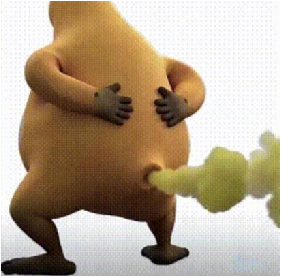
\includegraphics[width=114.58bp,height=0.76\textheight,keepaspectratio]{figures/chapter06/figure06_12.pdf}
  \renewcommand{\thefigure}{6.12}
  \caption{正在发动沼气动力的奶蛙}
  \label{fig:06-12}
\end{figure}


奶蛙的招牌雷霆动图动作之一。放屁的奶蛙会左右开弓连续释放气体，最后以一发蓄力的巨响收尾。
